\subsection{SinCos Interface}\label{subsec:SinCos_Interface}
Wie in Kapitel \ref{subsubsec:Resolver} beschrieben wurde, benötigt der Resolver ein Sinus-Signal, welches als Referenzsignal für die Sin- und Cos-Spule dient. Ebenso muss das zurückkehrende Signal gefiltert und Verstärkt werden.
Dazu wird auf ein Resolver-Interface der Firma NXP zurückgegriffen. Dieses hat drei ein Verstärker-Schaltkreise. Der erste ist der Sinus erzeugende Schaltkreis, die beiden anderen sind Filter- und Verstärkungsschaltkreis, jeweils einer für das Sinus- und Cosinus-Signal.

\subsubsection{Problem}\label{subsubsec:Problem_TMC6200}

Das zu lösende Problem besteht in der Transformation eines Rechtecksignals, welches vom Mikrocontroller gegeben wird, in ein Sinussignal, welches für den Resolver gebraucht wird. Der Verstärkerschaltkreis für die rückkehrenden Signale muss gewährleisten, dass das Signal in einem Bereich von 1..4V liegt. Dafür benötigt das Signal einen Offset von 2.5V.

\subsubsection{Schaltungsaufbau}\label{subsubsec:Schaltungsaufbau_TMC6200}

Der Opamp \textbf{IC700 A} transformiert das Rechtecksignal mittels Integrator in ein Dreiecksignal. Der Opamp \textbf{IC700 B} integriert das Dreiecksignal erneut und erzeugt ein sinusähnliches Signal.
Die Widerstandsverhältnisse \textbf{R1/R3} und \textbf{R2/R4} beeinflussen die Linearität des Integrators. Je höher dieses Verhältnis ist, desto besser wird das Sinussignal am Ausgang. Ist das Verhältnis zu hoch, wird die Schaltung störungsanfällig gegen das eingespiesene Rechtecksignal und gegen das PWM-Signal der H-Brücke. Um ein Signal mit hoher Qualität zu erreichen, sollte der Duty-Cycle des Eingangssignals genau 50\% betragen.

Das Dreiecksignal soll innert einer halben Periodentdauer um drei Volt steigen. Das heisst es ergibt sich gemäss Formel \ref{equ:Anstiegsrate_U1A} eine Anstiegsrate von 0.048V/\textmu s.
Der auf 5.6nF dimensionierte Kondensator wird so gemässs Formel \ref{equ:Strom_C1} einen maximalen Strom von 269 \textmu A leiten.

\begin{equation}
Anstiegsrate = \frac{\Delta_U}{T/2} = \frac{3V}{62.5 \mu s} = 0.048\frac{V}{\mu s}
\label{equ:Anstiegsrate_U1A}
\end{equation}

\begin{equation}
I_{C1} = C1 \cdot Anstiegsrate = 5.6 \cdot 10^{-9} \cdot 0.048\frac{V}{10^{-6}s} = 269\mu A
\label{equ:Strom_C1}
\end{equation}

So kann gemäss Formel \ref{equ:Dimensionierung_R1} der Widerstand R1 dimensioniert werden. Dessen Wert beträgt ungefähr 9300\textOmega.

\begin{equation}
R1 = \frac{\pm  2.5V}{I_C} = \frac{\pm 2.5V}{269 \mu A} = 9293.68 \textOmega
\label{equ:Dimensionierung_R1}
\end{equation}

Die Spule am Referenzsignal hat einen ohmischen Widerstand von 55\textOmega, was gemäss Formel \ref{equ:Spulenstrom}zu einem Spitzenstrom von 90mA ergibt.

\begin{equation}
\^{I}_{Spule} = \frac{\^{U}_{Spule}}{R_{Spule}} = \frac{5V}{55\textOmega} = 0.09A = 90mA
\label{equ:Spulenstrom}
\end{equation}

Abbildung \ref{fig:Simulation_Referenzsignal} zeigt die Opamp-Schaltung für das Referenzsignal.

\begin{figure}[h!]
	\centering
	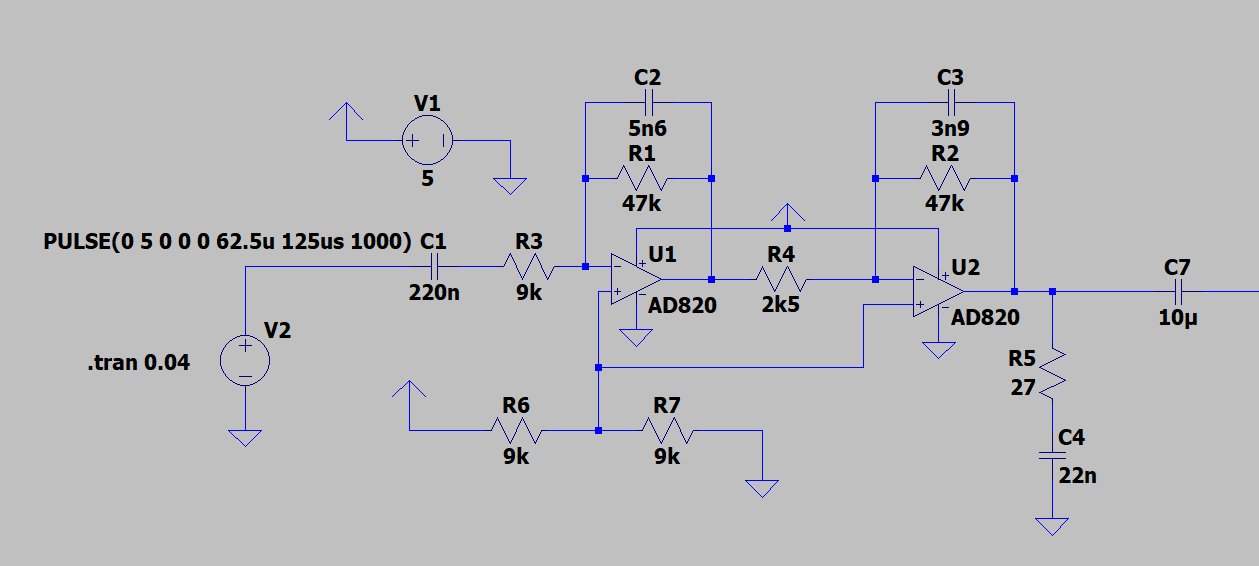
\includegraphics[width=0.8\textwidth]{graphics/Simulation_Schema_Referenzsignal.png}
	\caption{Schema Simulation Referenzsignal.}
	\label{fig:Simulation_Referenzsignal}
\end{figure}

Die passiven Elemente \textbf{R700/C701} verhindern ein Schwingen des Ausgangs, wenn induktive Lasten angetrieben werden.

Der Kondensator \textbf{C700} entkoppelt das Ausgangssignal.

Beide Operationsverstärker werden mit Single-Supply versorgt, weshalb ein virtueller Ground erstellt wird mit den Widerständen \textbf{R704 und R706}. So Pendelt das Signal um die 2.5V Referenzspannung. Erwünscht ist ein Ausgangssignal zwischen 0 und 5 V, das heisst, dass eine Amplitude von 2.5 angestrebt wird.

Die Schaltung wurde in LTSpice aufgebaut, um das Verhalten zu untersuchen. Folgende Resultate wurden erzielt:

Wird nun ein Rechtecksignal eingespiesen, wird dieses Integriert. Abbildung \ref{fig:Simulation_Rechteck_Dreieck} zeigt das Rechtecksignal und das daraus resultierende Dreiecksignal.

\begin{figure}[h!]
	\centering
	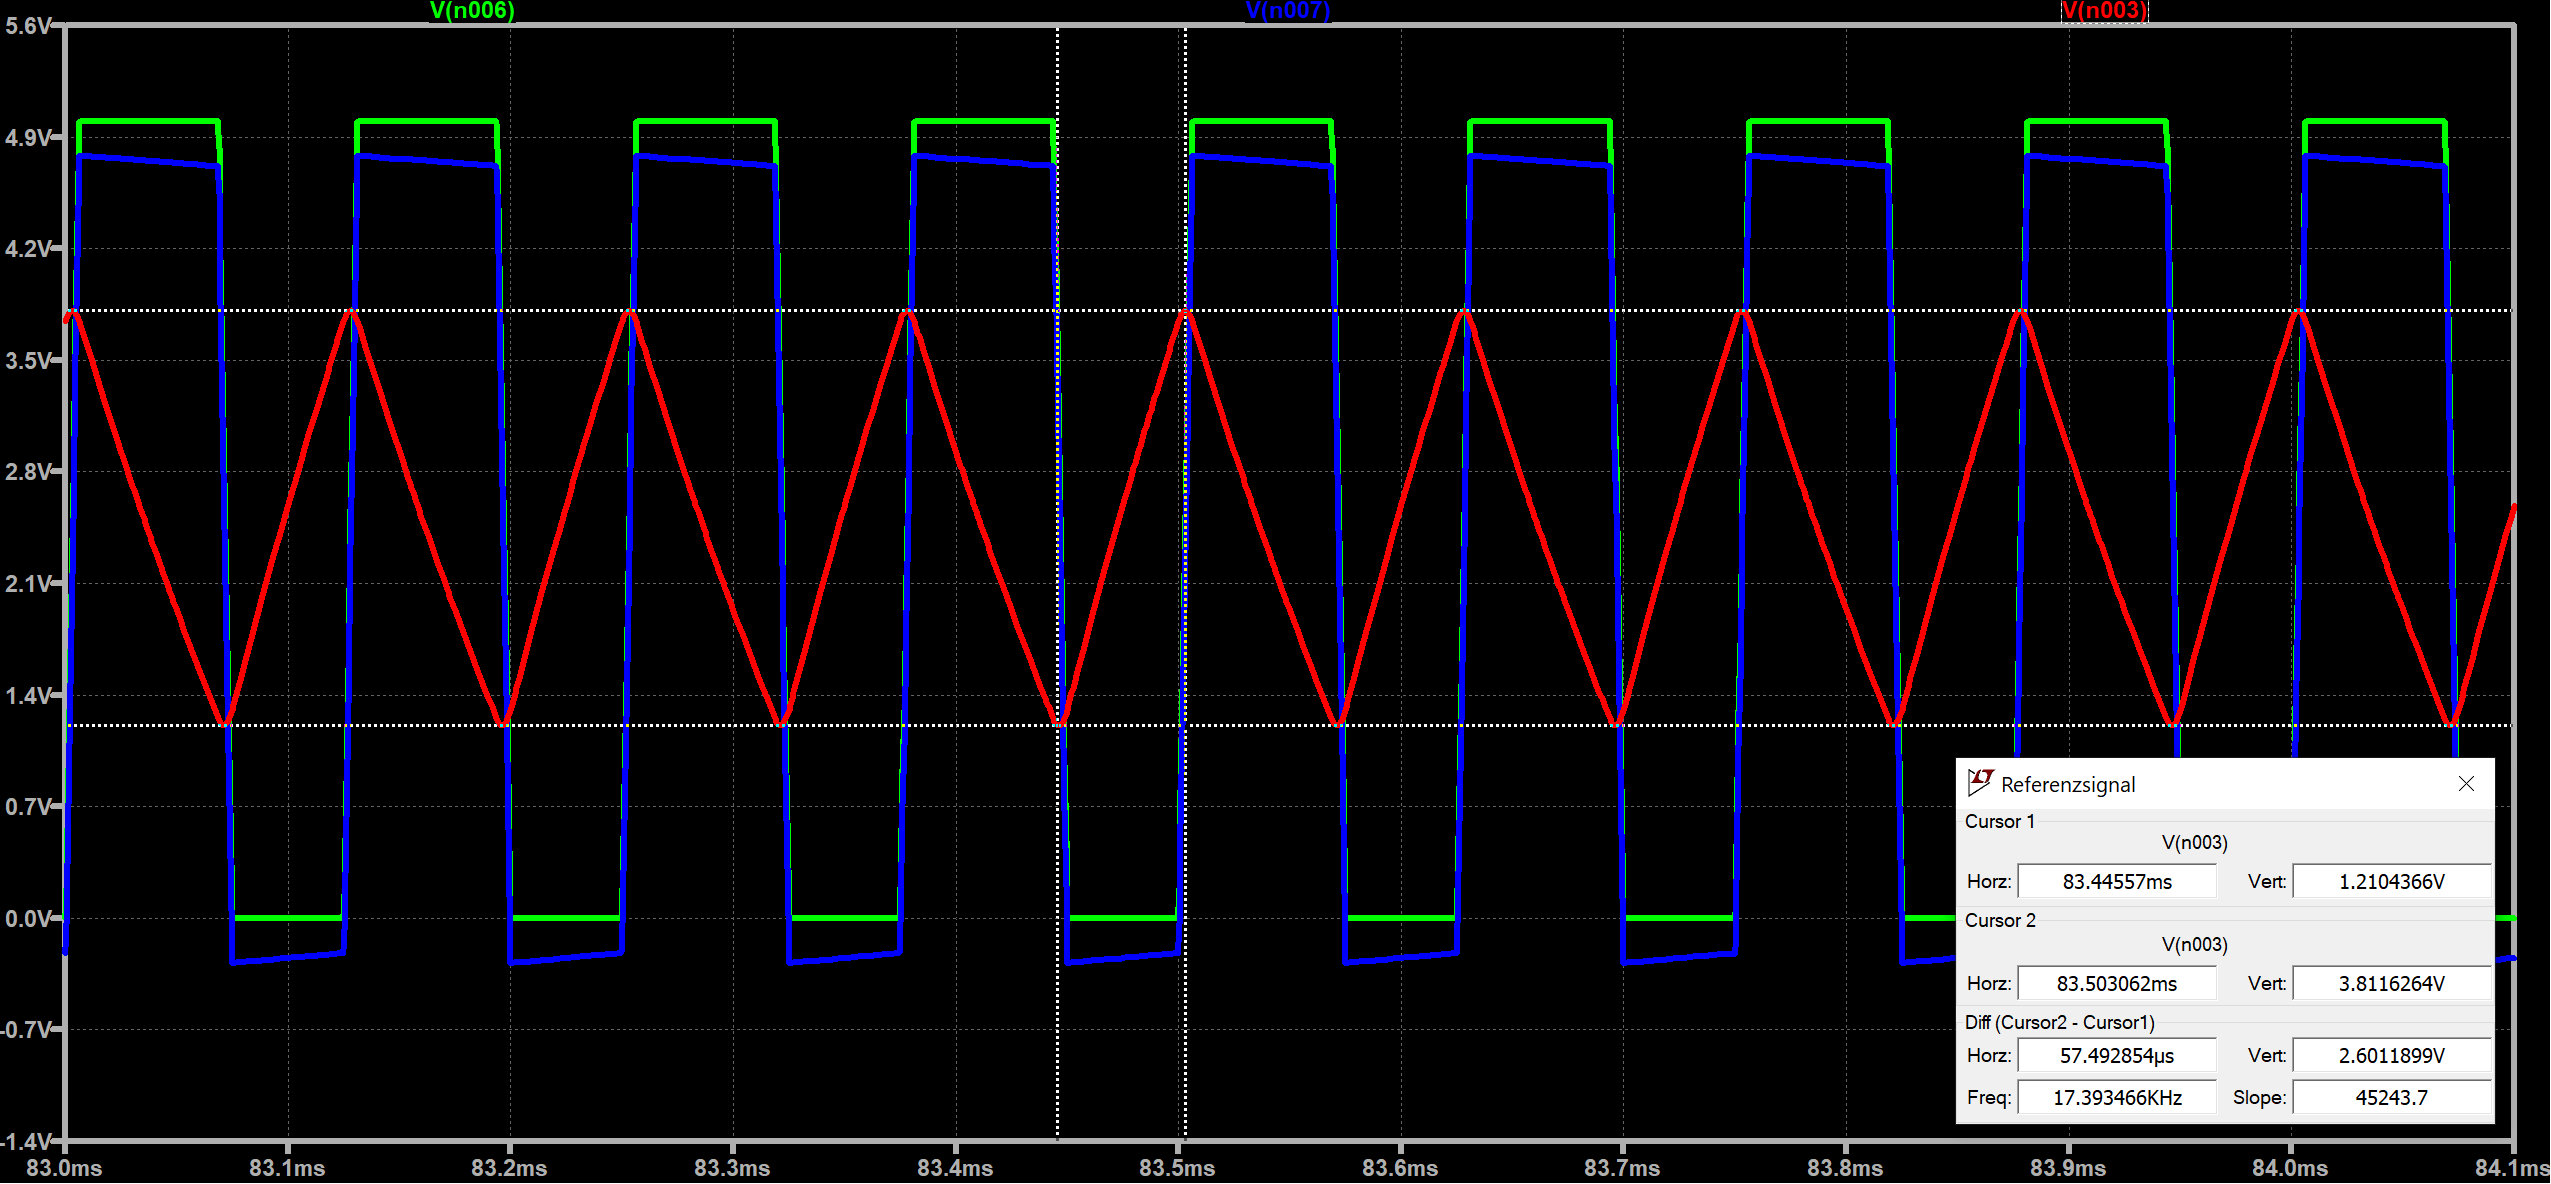
\includegraphics[width=0.6\textwidth]{graphics/Simulation_Signal_Viereck_Dreieck.png}
	\caption{Signale, wie sie gemäss Abbildung \ref{fig:Simulation_Referenzsignal} auftreten. Grün: Eingangs-PWM vom Mikrocontroller, Rot: Ausgangssignal zwischen Opamp U1 und Widerstand R4.}
	\label{fig:Simulation_Rechteck_Dreieck}
\end{figure}

Abbildung \ref{fig:Simulation_Dreieck_Sinus} zeigt das Sinussignal (grün), welches aus dem Dreieck generiert wurde. Sie zeigt ebenfalls das Signal, wie es aus dem Resolver zurückgegeben würde.

\begin{figure}[h!]
	\centering
	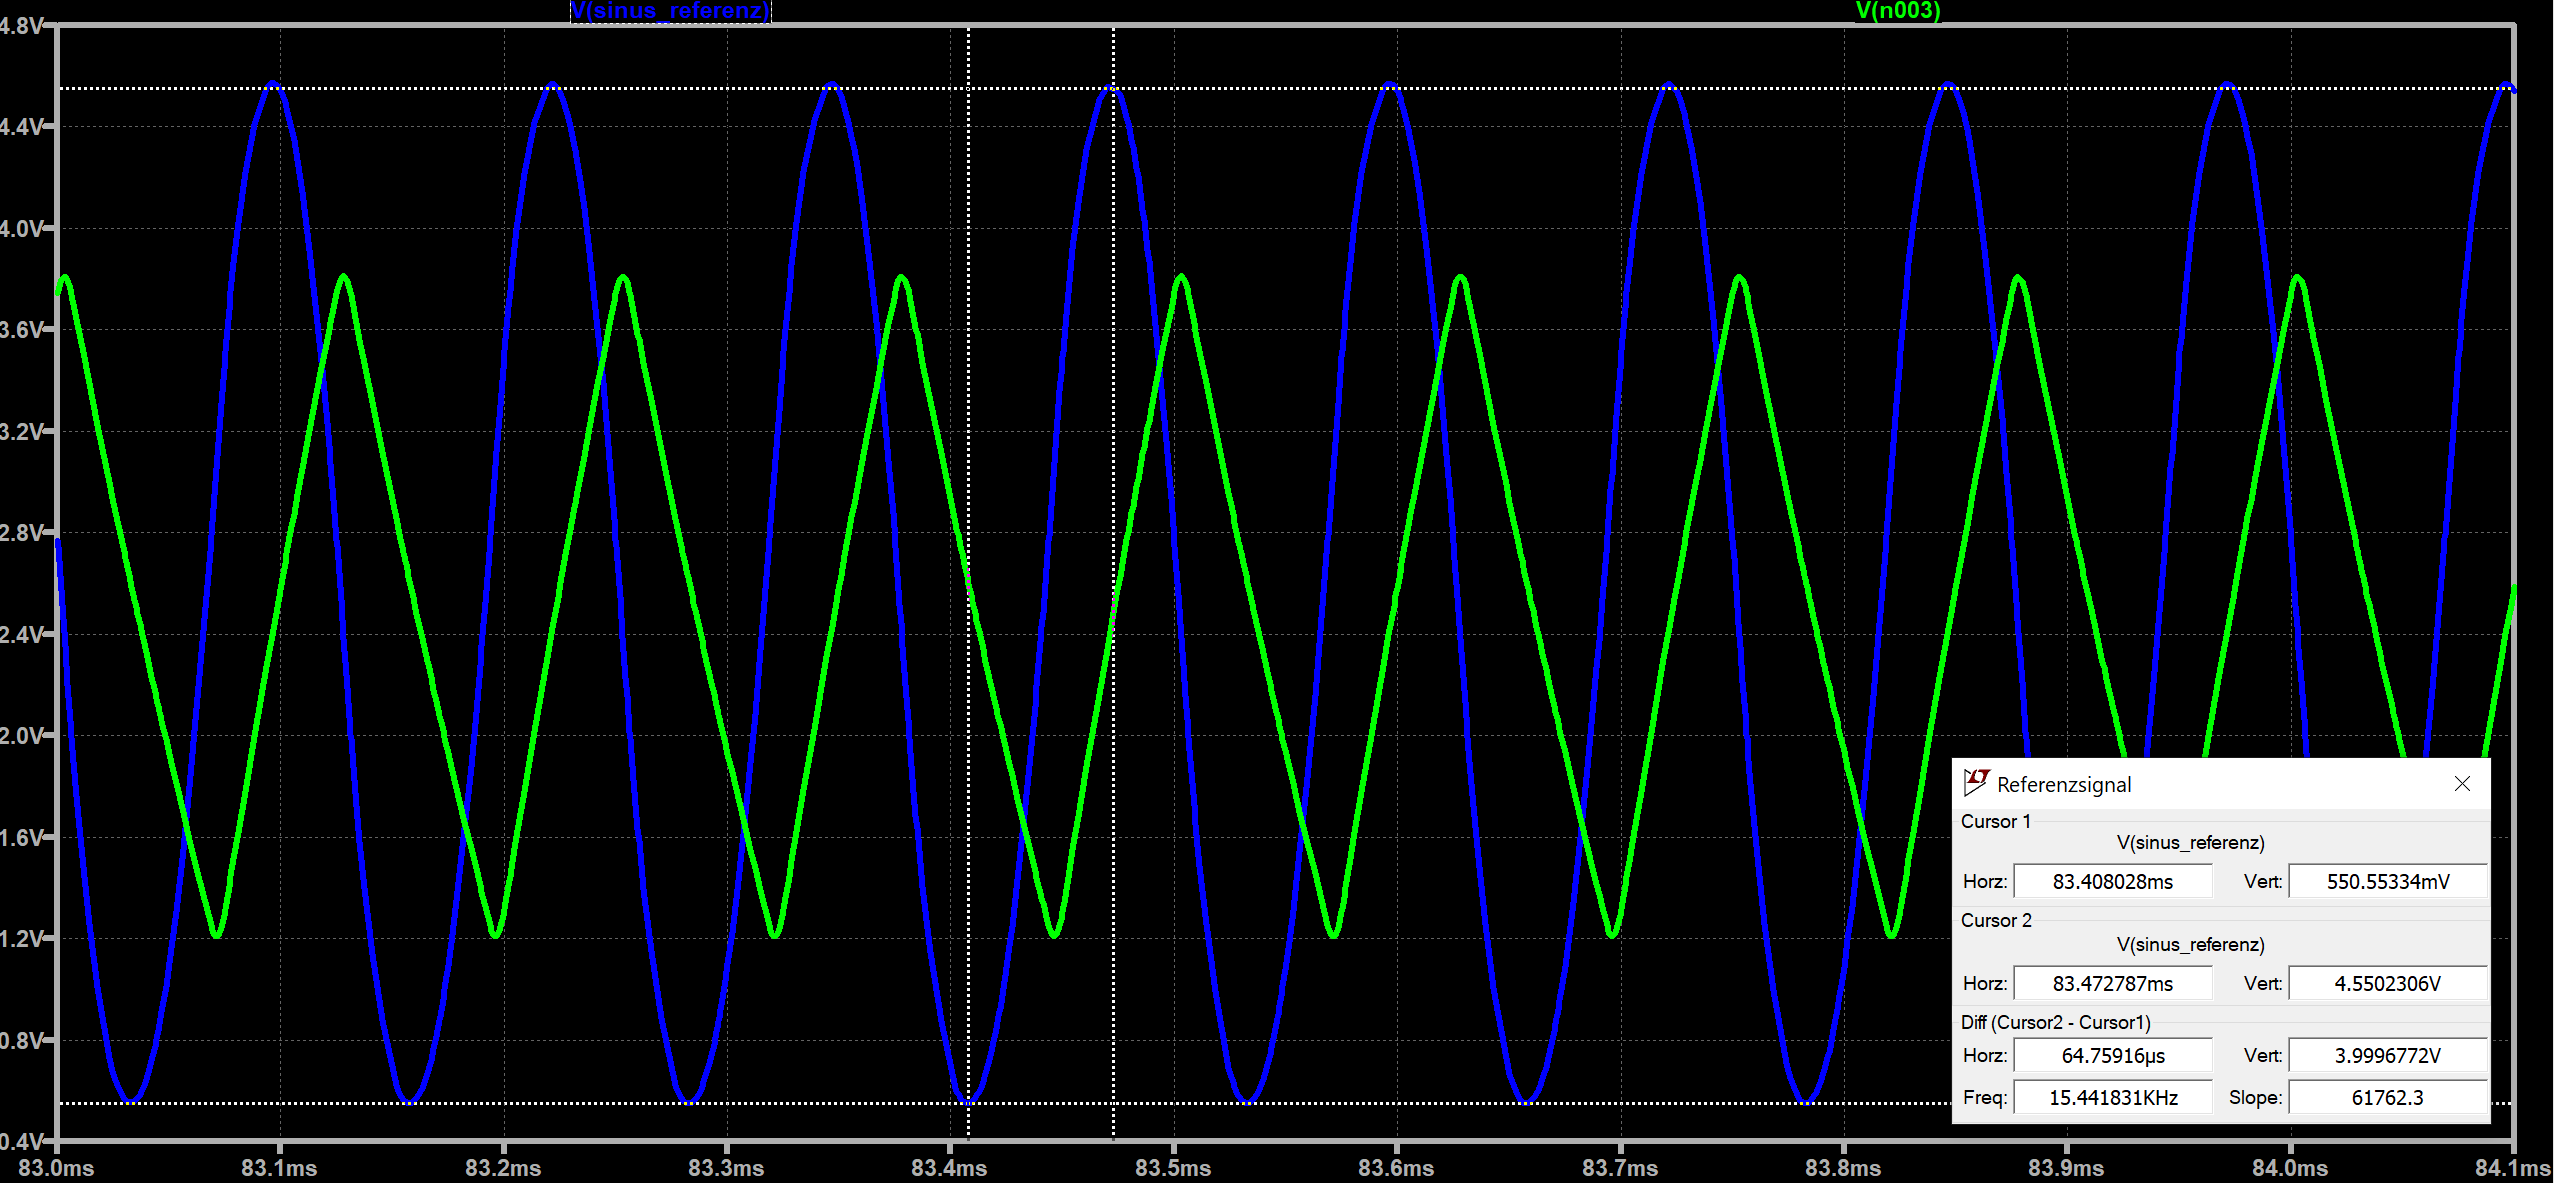
\includegraphics[width=0.6\textwidth]{graphics/Simulation_Signal_Sinus1_Sinus2.png}
	\caption{Signale, wie sie gemäss Abbildung \ref{fig:Simulation_Referenzsignal} auftreten. Grün: Sinus, welcher aus dem Dreiecksignal generiert wurde, Rot: Zurückkehrendes Signal aus Resolver mit einem Verhältnis von 2:1.}
	\label{fig:Simulation_Dreieck_Sinus}
\end{figure}

Die Abbildung \ref{fig:Simulation_Verstaerkungssignal} zeigt die Opamp-Schaltung für das zu verstärkende Signal, welches aus dem Resolver zurückkommt. Es soll so verstärkt werden, die Amplituden im Bereich von 1..4V liegen.

\begin{figure}[h!]
	\centering
	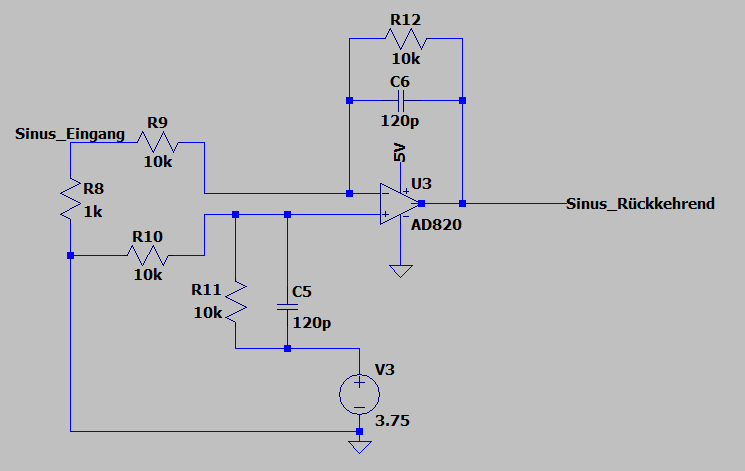
\includegraphics[width=0.6\textwidth]{graphics/Simulation_Schema_Verstaerkungssignal.png}
	\caption{Schema Simulation Verstärkungssignal.}
	\label{fig:Simulation_Verstaerkungssignal}
\end{figure}

Die Abbildung \ref{fig:Simulation_Sinus2_Sinus3} zeigt die Signale, wie sie in die Verstärkungsschaltung hineingehen und wie sie vertärkt und mit einem DC-Offset versehen werden.

\begin{figure}[h!]
	\centering
	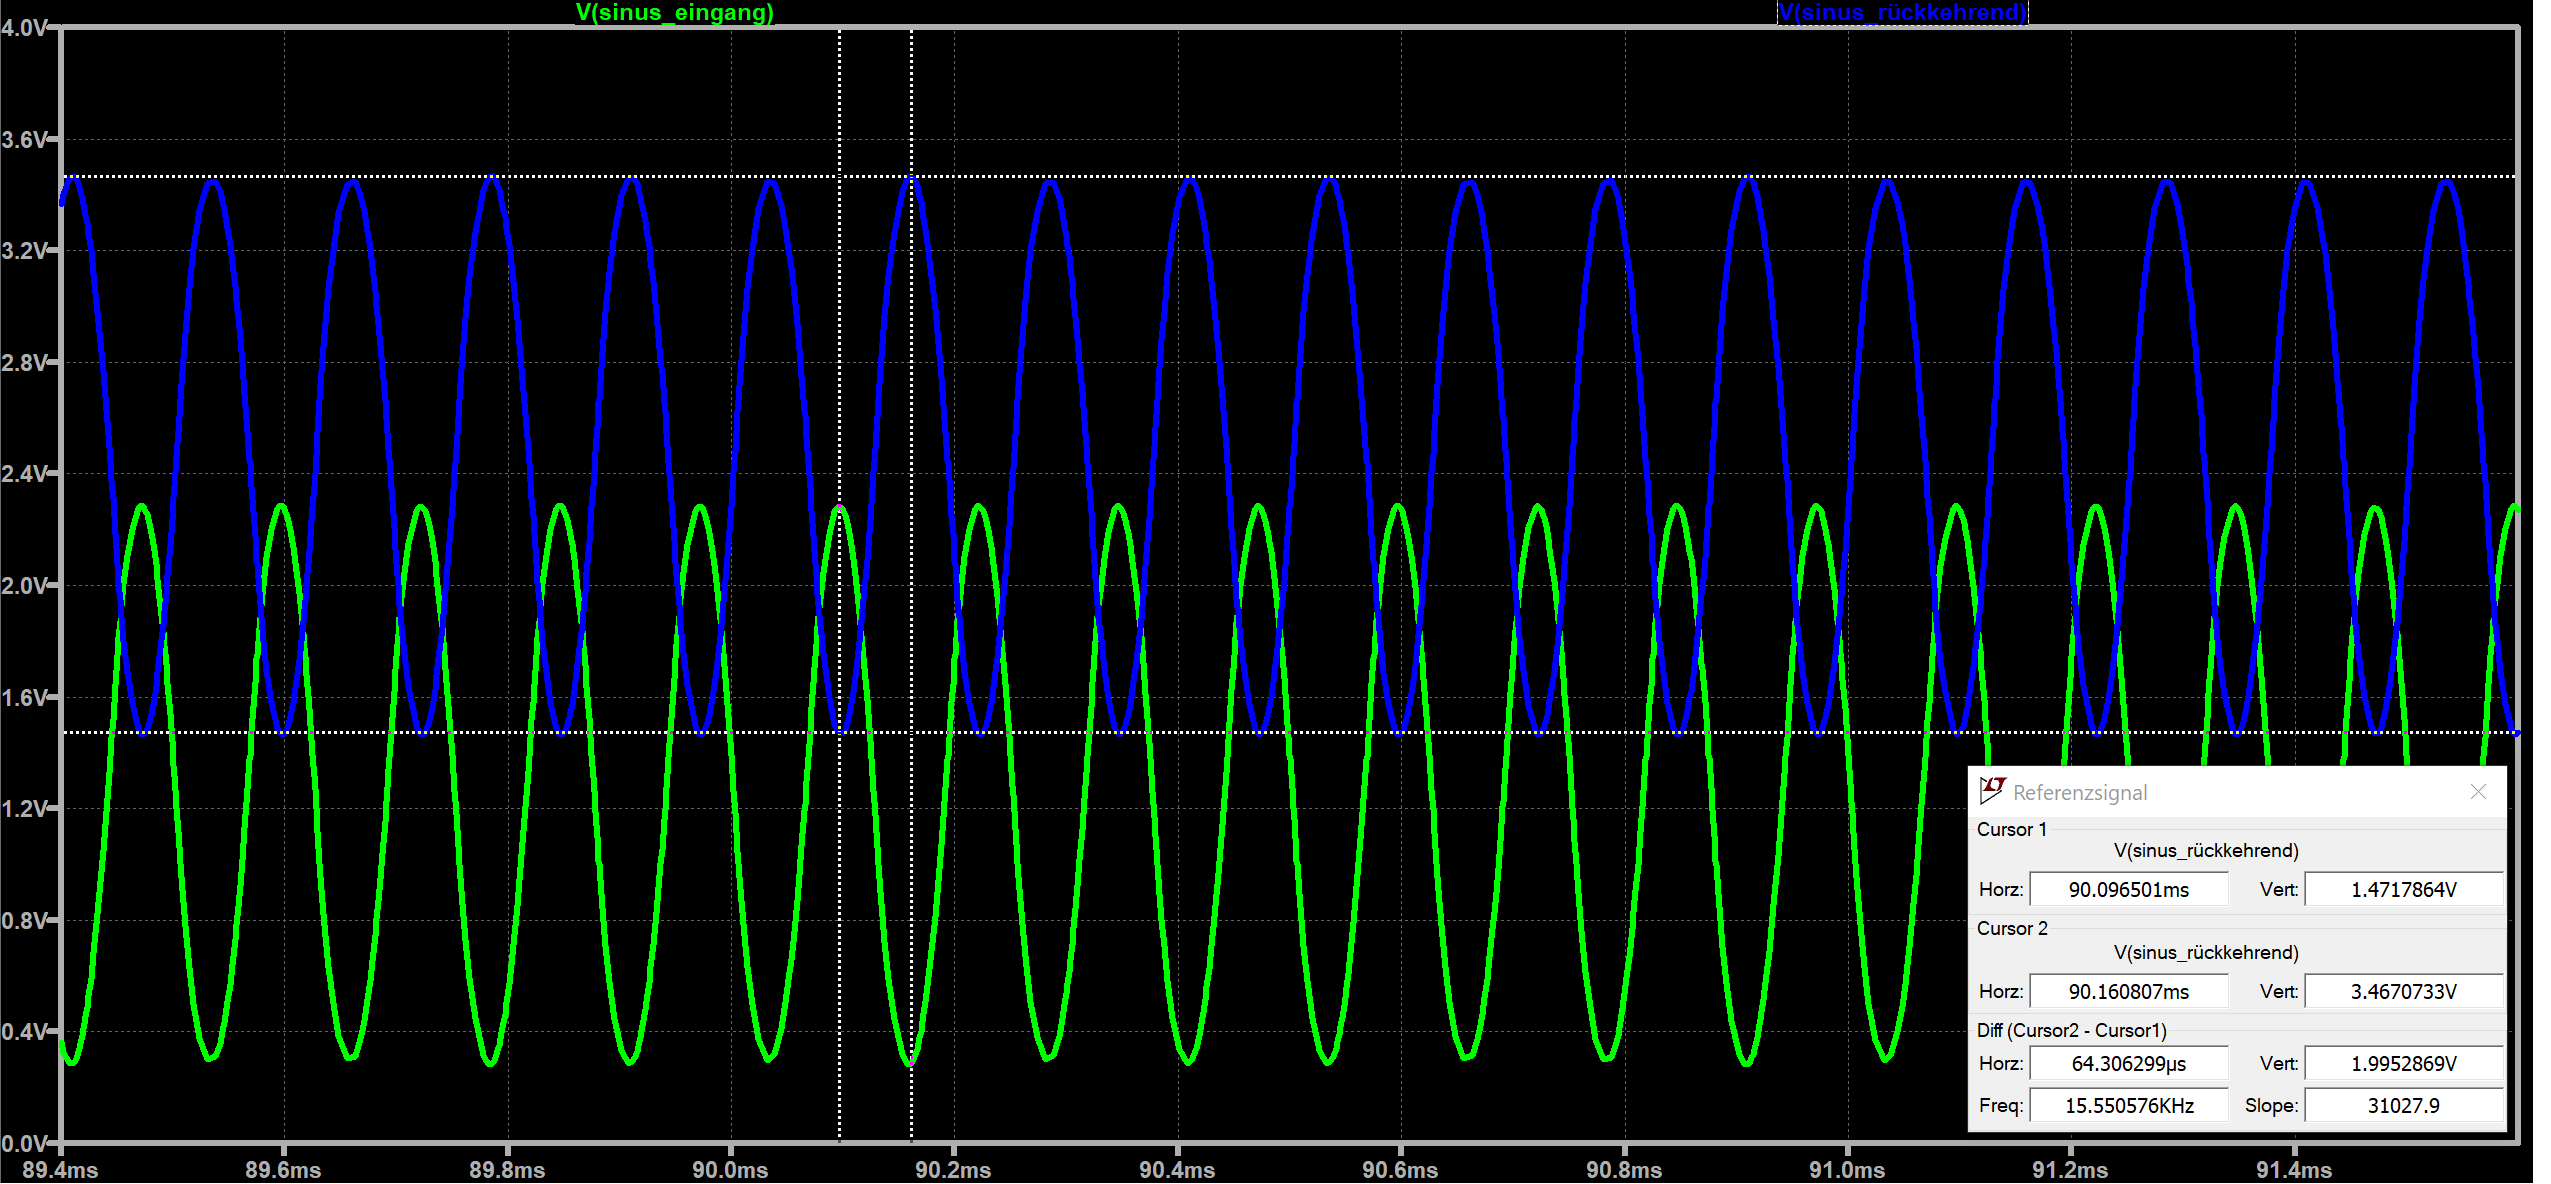
\includegraphics[width=0.6\textwidth]{graphics/Simulation_Sinus2_Sinus3.png}
	\caption{Signale, wie sie gemäss Abbildung \ref{fig:Simulation_Verstaerkungssignal} auftreten würden. Grün: Signal, welches für den TMC4671 verstärkt wurde. Rot: Signal, welches vom Resolver zurückkommt.}
	\label{fig:Simulation_Sinus2_Sinus3}
\end{figure}